\chapter{Laboratorio de pruebas}
\label{chapter6}

% **************************** Define Graphics Path **************************
\ifpdf
    \graphicspath{{Chapter6/Figs/Raster/}{Chapter6/Figs/PDF/}{Chapter6/Figs/}}
\else
    \graphicspath{{Chapter6/Figs/Vector/}{Chapter6/Figs/}}
\fi

Para validar funcionalmente el prototipo es preciso la construcción de un laboratorio de experimentación sobre el cual ejecutar un conjunto de pruebas e implementar algunos casos de uso representativos. Dentro de las pruebas funcionales se busca verificar aspectos importantes de la implementaci\'on como la clasificación de tr\'afico, el algoritmo de ruteo dinámico y el algoritmo de distribución de etiquetas.

Por otro lado con la implementaci\'on de algunos casos de uso representativos se busca validar la utilización del enfoque OpenFlow/SDN en la construcci\'on a futuro de la RAU2.\\

El siguiente capitulo esta destinado a la presentación del laboratorio de pruebas construido y a la descripción de las diferentes pruebas realizadas.

% **************************** Construccion del TestBed ************************** 
\section{Definición del Laboratorio}

Como se menciona anteriormente uno de los objetivos de este laboratorio de experimentaci\'on es verificar el correcto funcionamiento de la implementaci\'on realizada, en particular en los aspectos críticos de la misma como la capacidad para clasificar trafico y los diferentes algoritmos de ruteo, distribución de etiquetas, actualización topologica, etc. 

Para esto es necesario construir un prototipo con suficientes nodos y enlaces como para poder definir varios servicios de redes privadas. Tambi\'en interesa la existencia de caminos alternativos entre un par de nodos origen y destino para poder comprobar el funcionamiento del algoritmo de ruteo y evaluar el comportamiento del prototipo cuando la topolog\'ia cambia, desconectando enlaces, apagando nodos, etc.\\

Teniendo en cuanta los requerimientos mencionados se construye un laboratorio de pruebas con la siguiente topolog\'ia (ver figura \ref{fig:LaboratorioDePruebasTopo}).
  
\begin{figure}[ht!] 
\centering    
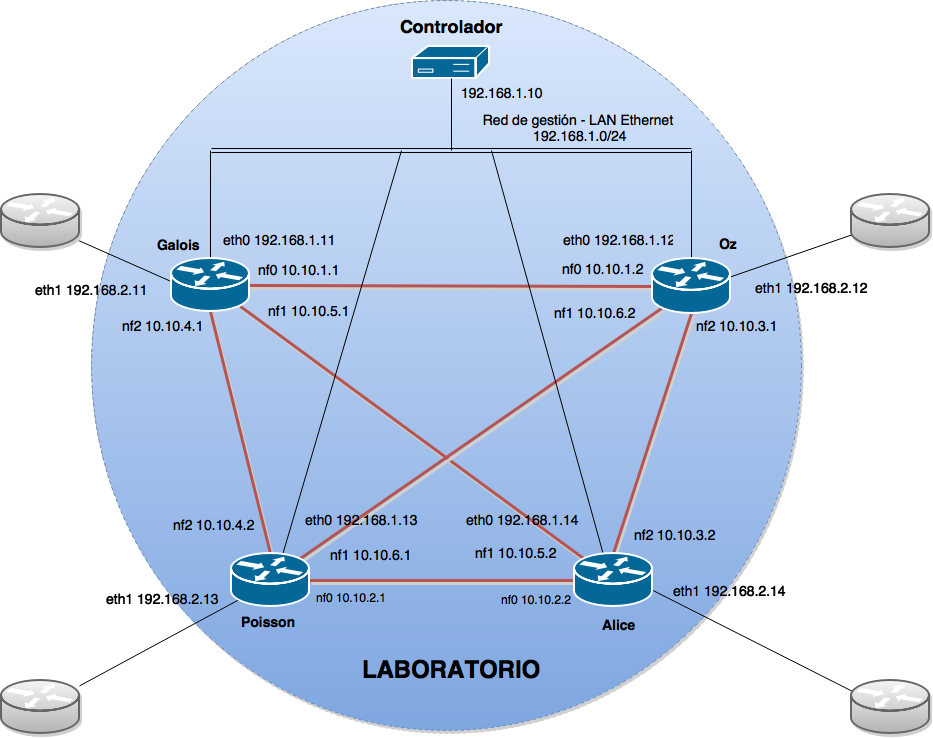
\includegraphics[width=0.85\textwidth]{Topologia}
\caption[Laboratorio de pruebas - Topolog\'ia]{Laboratorio de pruebas - Topolog\'ia}
\label{fig:LaboratorioDePruebasTopo}
\end{figure}

El laboratorio se compone de cuatro nodos implementados en base al dispositivo RAU-Switch conectados entre si con enlaces de fibra \'optica multimodo. Cada nodo esta conectado a los otros tres nodos de la topolog\'ia implementando de esta forma una topolog\'ia full mesh de cuatro nodos.

A su vez cada nodo esta conectado al controlador SDN del prototipo mediante una interfaz de red de 10Mb (interfaces \textbf{eth0}).\\

Por la forma que tiene la topolog\'ia, los cuatro nodos nombrados \textit{Galois}, \textit{Poisson}, \textit{Oz} y \textit{Alice} son nodos de borde. Esto quiere decir que RAUFlow los considera como nodos habilitados para ser nodo de ingreso \'o nodo de egreso en la definici\'on de servicios de redes privadas.

Por otro lado cada nodo cuenta con una interfaz de red de 100Mb (interfaz \textbf{eth1}) utilizada como interfaz externa para la conexi\'on con otras subredes. Estas interfaces son utilizadas por RAUFlow para la definici\'on de servicios de VPN como los puntos de entrada y salida de tr\'afico. Por tanto cada una de estas interfaces se encuentra directamente conectada a la subred de una VPN en particular.\\  

Como se menciona anteriormente en lacp\'itulo 5, la representaci\'on utilizada para modelar una topolog\'ia de red es la de un multigrafo dirigido ponderado. En la figura \ref{fig:LaboratorioDePruebasCostos} se muestra esta representaci\'on para la topolog\'ia del prototipo. Como puede apreciarse en la im\'agen cada enlace tiene su respectivo costo asociado.

Por simplicidad en el diagrama se han obviado los enlaces existentes entre el Controlador y cada uno de los nodos. Como se menciona en el cap\'itulo 4 la instancia de Quagga ejecutada en el controlador tiene como \'unico objetivo contar con un acceso local a la LSDB. Por ello conceptualmente el costo asociado a cada uno de estos enlaces es infinito, lo cual en pr\'actica se realiza asignando el valor 65535.  

\begin{figure}[ht!] 
\centering    
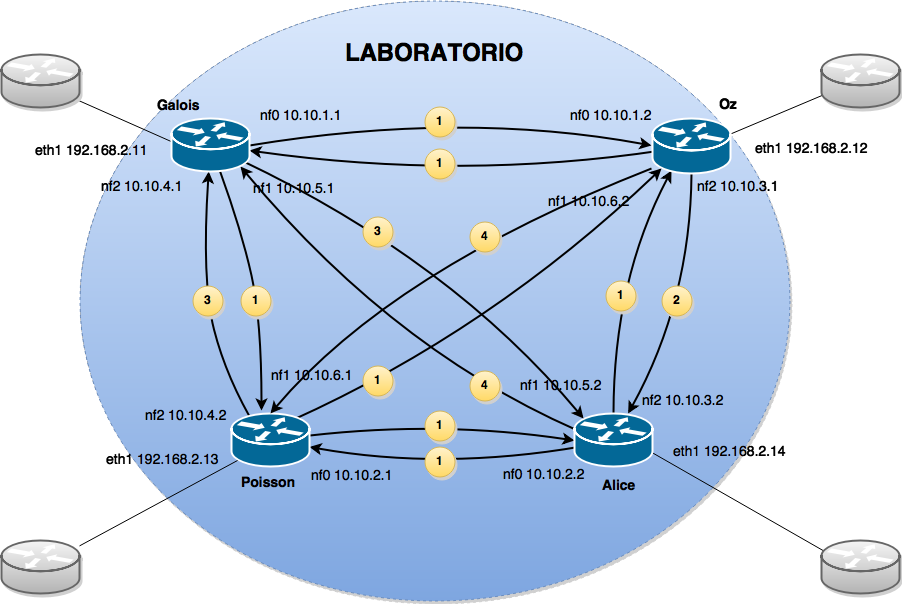
\includegraphics[width=0.85\textwidth]{TopologiaCostos}
\caption[Laboratorio de pruebas - Costos de la topolog\'ia]{Laboratorio de pruebas - Costos de la topolog\'ia}
\label{fig:LaboratorioDePruebasCostos}
\end{figure}

Sobre este laboratorio se implementan dos casos de uso representativos: (a) VPN de capa 3 y (b) VPN de capa 2. Sobre cada uno de estos casos de uso a su vez se ejecutan una serie de pruebas orientadas a verificar el correcto funcionamiento de las componentes m\'as importantes en la implementaci\'on de RAUFlow y RAU-Switch.

A continuaci\'on se describen los resultados obtenidos en la implementaci\'on de estos casos de uso y la ejecuci\'on de estas pruebas, comenzando por el caso de uso VPN de capa 3.

\section{VPN de capa 3}

Las redes privadas virtuales de capa 3 son un tipo de servicio comunmente brindado por un operador de red y es en particular uno de los servicios que se quiere implementar en la RAU2. En particular sobre este tipo de redes privadas puede implementarse clasificaci\'on de tr\'afico por tipo de aplicaci\'on o numeraci\'on de capa 3 por ejemplo.\\

En este trabajo se implementan dos escenarios diferentes para este tipo de red privada: (a) red privada multipunto con una \'unica organizaci\'on y tres sucursales f\'isicamente separadas, (b) red privada punto a punto con dos organizaciones, cada una de ellas con dos sucursales f\'isicamente separadas.

A continuaci\'on se detalla la construcci\'on de ambos escenarios y los resultados obtenidos.

\subsection{Escenario 1 - Red Privada Multipunto}

Este escenario representa una red privada multipunto de capa 3. En el mismo se tiene una sola organizaci\'on o red privada dividida en 3 sucursales o subredes físicamente separadas.

\begin{figure}[ht!] 
\centering    
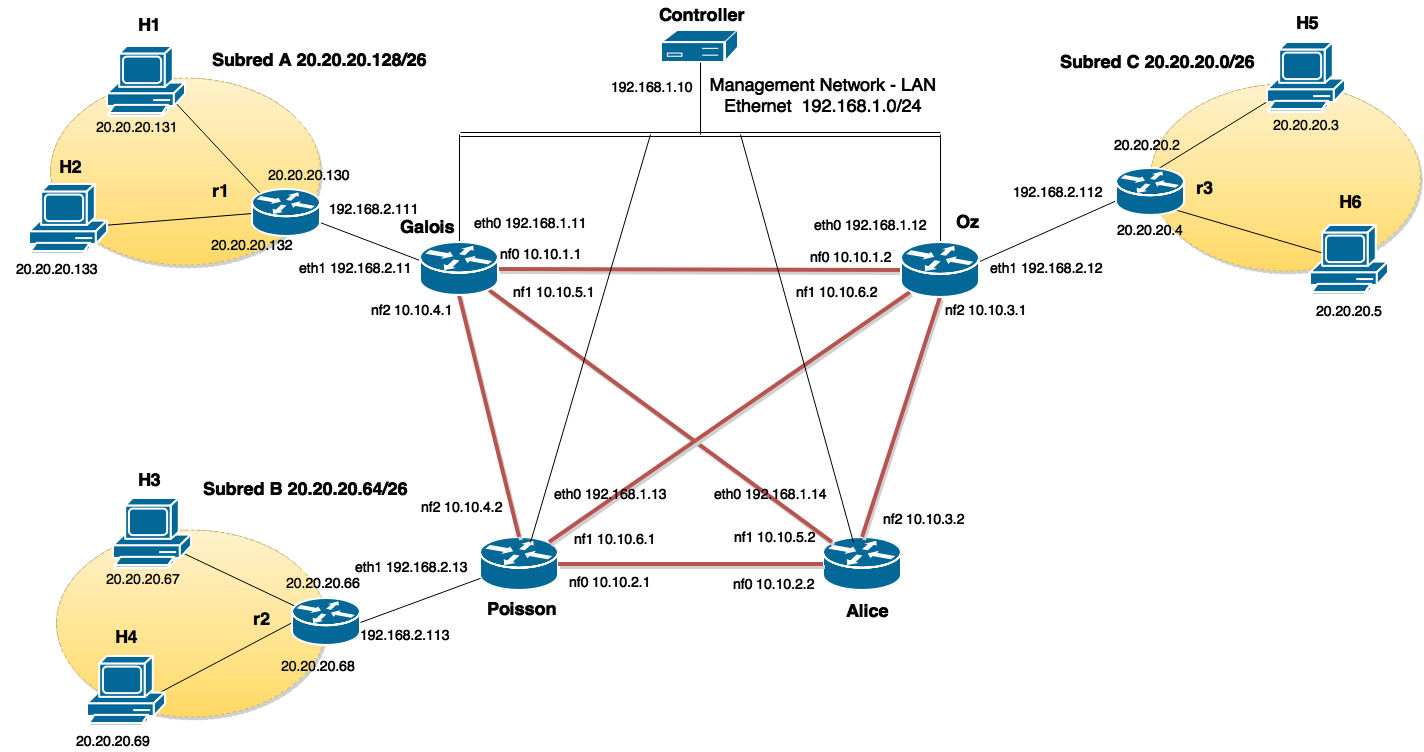
\includegraphics[width=1.0\textwidth]{CU1P1}
\caption[VPN de capa 3 - Escenario 1]{VPN de capa 3 - Escenario 1}
\label{fig:CUP1}
\end{figure}

Sobre este escenario se ejecutan una serie de pruebas orientadas a verificar los siguientes aspectos relacionados al prototipo:

\begin{enumerate}
\item Algoritmo de ruteo
\item Algoritmo de distribución de etiquetas
\item Clasificaci\'on de tr\'afico
\item Actualizaci\'on de rutas cuando cambia la topolog\'ia
\item Capacidad para crear VPN multipunto
\end{enumerate}

Para construir la red privada multipunto uniendo las tres subredes mencionadas y adem\'as verificar los puntos anteriores, se instancian los siguientes servicios(ver tabla \ref{table:TablaFlujos}). Por cada par de subredes se crean dos servicios (un servicio para cada sentido del tr\'afico).\\

\newpage
\begin{table}[h]
\begin{tabular}{| l | l | l | p{4cm} | p{4cm} |}
\hline
Nombre & Ingreso & Egreso & Clasificación & Descripción \\ \hline

\crule[Aquamarine]{0.3cm}{0.3cm} S1 & Galois - eth1 & Oz - eth1 & ip\_src=20.20.20.128/26 ip\_dst=20.20.20.0/26 eth\_type=0x0800 & Tr\'afico IP de Subred A a Subred C \\ \hline

\crule[Red]{0.3cm}{0.3cm} S2 & Oz - eth1 & Galois - eth1 & ip\_src=20.20.20.0/26 ip\_dst=20.20.20.128/26 eth\_type=0x0800 & Tr\'afico IP de Subred C a Subred A \\ \hline

\crule[ForestGreen]{0.3cm}{0.3cm} S3 & Galois - eth1 & Poisson - eth1 & ip\_src=20.20.20.128/26 ip\_dst=20.20.20.64/26 eth\_type=0x0800 & Tr\'afico IP de Subred A a Subred B \\ \hline

\crule[LimeGreen]{0.3cm}{0.3cm} S4 & Poisson - eth1 & Galois - eth1 & ip\_src=20.20.20.64/26 ip\_dst=20.20.20.128/26 eth\_type=0x0800 & Tr\'afico IP de Subred B a Subred A \\ \hline

\crule[RoyalPurple]{0.3cm}{0.3cm} S5 & Poisson - eth1 & Oz - eth1 & ip\_src=20.20.20.64/26 ip\_dst=20.20.20.0/26 eth\_type=0x0800 IP & Tr\'afico de Subred B a Subred C \\ \hline

\crule[YellowOrange]{0.3cm}{0.3cm} S6 & Oz - eth1 & Poisson - eth1 & ip\_src=20.20.20.0/26 ip\_dst=20.20.20.64/26 eth\_type=0x0800 & Tr\'afico IP de Subred C a Subred B \\ \hline \hline

S7 & Galois - eth1 & Oz - eth1 & arp\_tpa=192.168.2.112 eth\_type=0x0806 & Consultas ARP Subred A a Subred C \\ \hline

S8 & Oz - eth1 & Galois - eth1 & arp\_tpa=192.168.2.111 eth\_type=0x0806 & Consultas ARP Subred C a Subred A \\ \hline

S9 & Galois - eth1 & Poisson - eth1 & arp\_tpa=192.168.2.113 eth\_type=0x0806 & Consultas ARP Subred A a Subred B \\ \hline

S10 & Poisson - eth1 & Galois - eth1 & arp\_tpa=192.168.2.111 eth\_type=0x0806 & Consultas ARP Subred B a Subred A \\ \hline

S11 & Poisson - eth1 & Oz - eth1 & arp\_tpa=192.168.2.112 eth\_type=0x0806 & Consultas ARP Subred B a Subred C \\ \hline

S12 & Oz - eth1 & Poisson - eth1 & arp\_tpa=192.168.2.113 eth\_type=0x0806 & Consultas ARP Subred C a Subred B \\ \hline

\end{tabular}
\vspace{0.3cm}
\caption[CU1 - Escenario 1, servicios creados]{CU1 - Escenario 1, servicios creados}
\label{table:TablaFlujos}
\end{table}

Para cada uno de estos servicios adem\'as se indica el etherype 0x0800 correspondiente al tipo de tr\'afico IPv4.\\

De esta forma se implementa una VPN de capa 3 para la organizaci\'on mencionada, uniendo las tres sucursales. A continuaci\'on se detallan las pruebas realizadas para cada uno de los aspectos mencionados anteriormente.

\subsubsection{Verificaci\'on de Algoritmo de ruteo}
En esta secci\'on se eval\'ua el correcto funcionamiento del algoritmo de ruteo. Para ello se comparan los caminos computados por el algoritmo para cada servicio, con los respectivos mejores caminos te\'oricos(previamente calculados de forma manual). 

Para cada camino se verifican dos cosas: (1) que el camino calculado se corresponde con el camino te\'orico y (2) que el camino es correctamente instalado en forma de reglas de reenvío (en base a conmutaci\'on de etiquetas) en las respectivas tablas de flujos OpenFlow de cada nodo en el camino.\\

Como se ha mencionado, los caminos te\'oricos son calculados manualmente observando los costos de la topolog\'ia (figura \ref{fig:LaboratorioDePruebasCostos}). Los resultados de este procedimiento se muestran en la figura \ref{fig:CUP1Caminos}. Cada camino es identificado mediante el código de color de cada servicio.\\

\begin{figure}[ht!] 
\centering    
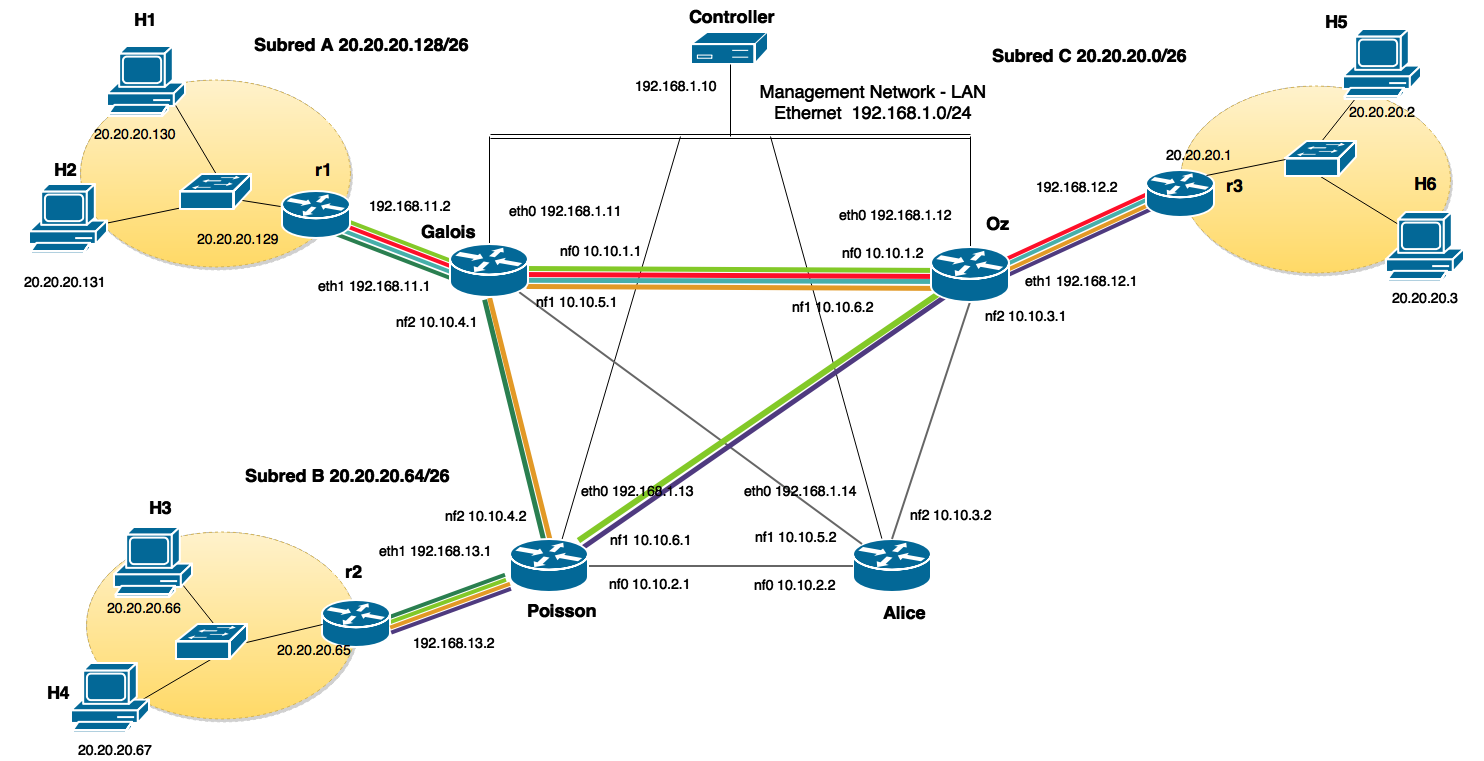
\includegraphics[width=1.0\textwidth]{CU1P1Caminos}
\caption[Escenario 1 - Caminos para servicios]{Escenario 1 - Caminos para servicios}
\label{fig:CUP1Caminos}
\end{figure}

Para obtener los caminos calculados por el algoritmo de ruteo, se analizan las tablas de flujos de Open vSwitch en cada nodo de la red del laboratorio. A partir del contenido de estas tablas fácilmente puede reconstruirse el camino previamente calculado.\\

En las figuras ~\ref{fig:CU1P1DumpFlows1}~-~\ref{fig:CU1P1DumpFlows4} se muestran las tablas de flujos asociadas a cada nodo del laboratorio. Para conseguir esta informaci\'on se utiliza el comando \textbf{dump-flows} de la herrmaienta Open vSwitch. Sin embargo puede obtenerse tambi\'en esta informaci\'on desde la propia interfaz gr\'afica de RAUFlow.\\

Asumiendose la notaci\'on $(n, i)$ para referirse a un enlace, donde \textit{n} indica nodo origen e \textit{i} interfaz de reenvío en \textit{n} para el próximo salto, entonces $<(n_1, i_1), \dots, (n_k, i_k)>$ puede usarse para denotar un camino en el laboratorio. De esta forma se pueden comparar f\'acilmente los caminos te\'oricos con los calculados.\\

Tomando como ejemplo el caso del servicio S3, el camino te\'orico puede denotarse de la siguiente forma:
 
$$<(Galois, nf_2)>$$

\begin{figure}[ht!] 
\centering    
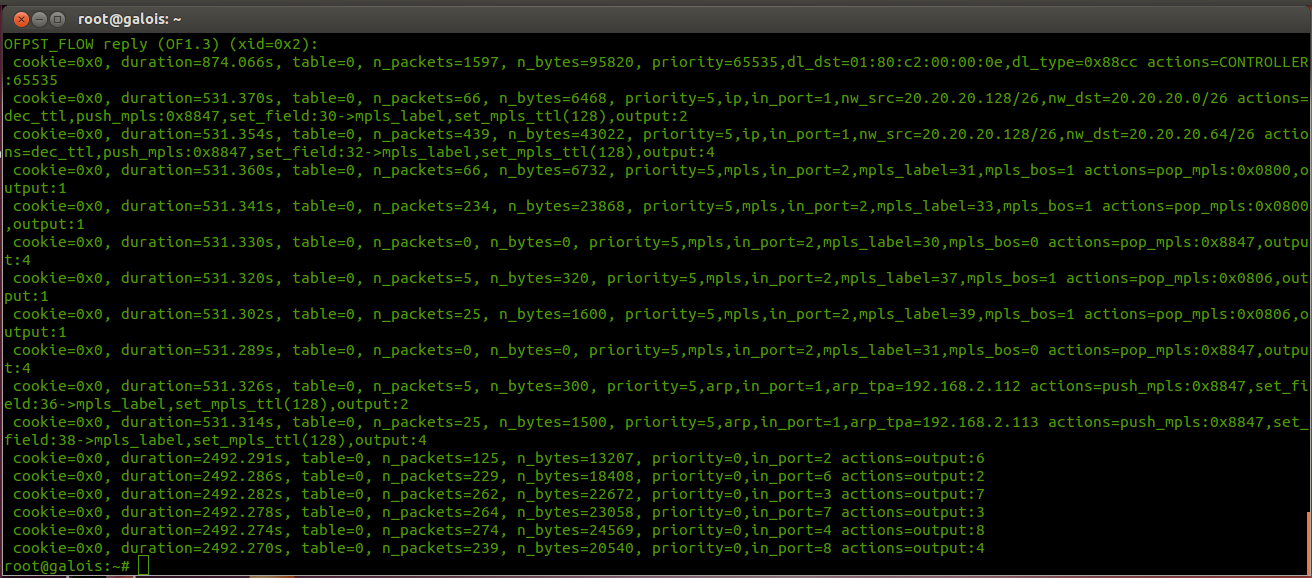
\includegraphics[width=1.0\textwidth]{LabE1P1Gal}
\caption[Tabla de flujos ovs - Galois]{Tabla de flujos ovs - Galois}
\label{fig:CU1P1DumpFlows1}
\end{figure}

\begin{figure}[ht!] 
\centering    
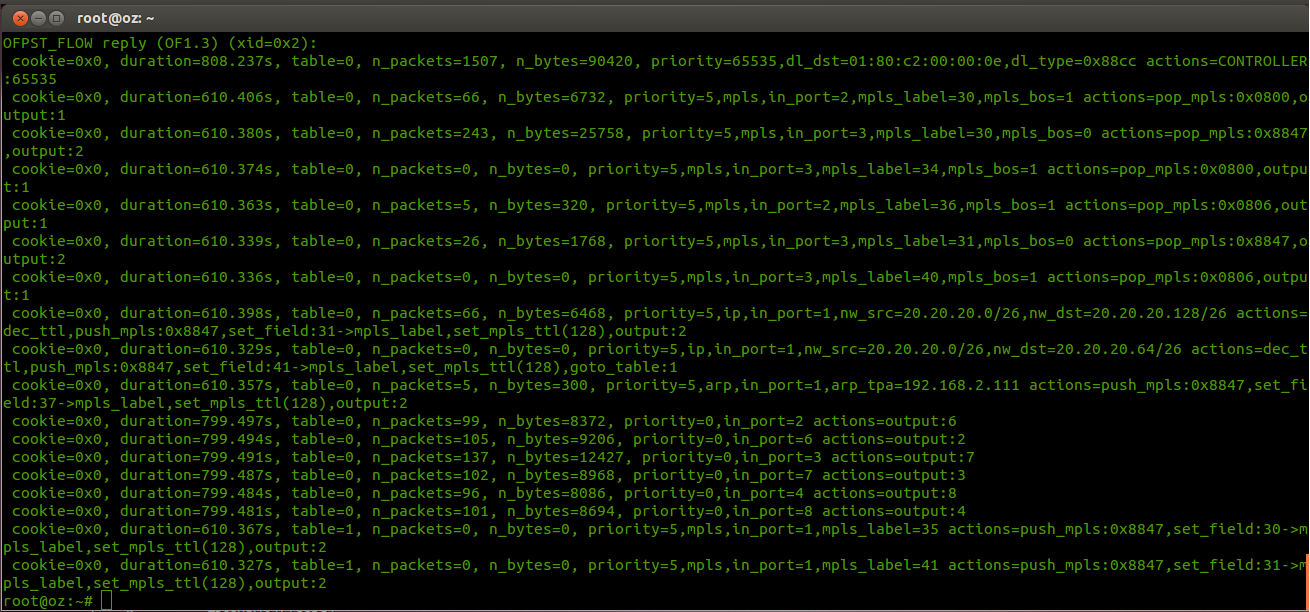
\includegraphics[width=1.0\textwidth]{LabE1P1Oz}
\caption[Tabla de flujos ovs - Oz]{Tabla de flujos ovs - Oz}
\label{fig:CU1P1DumpFlows2}
\end{figure}

\begin{figure}[ht!] 
\centering    
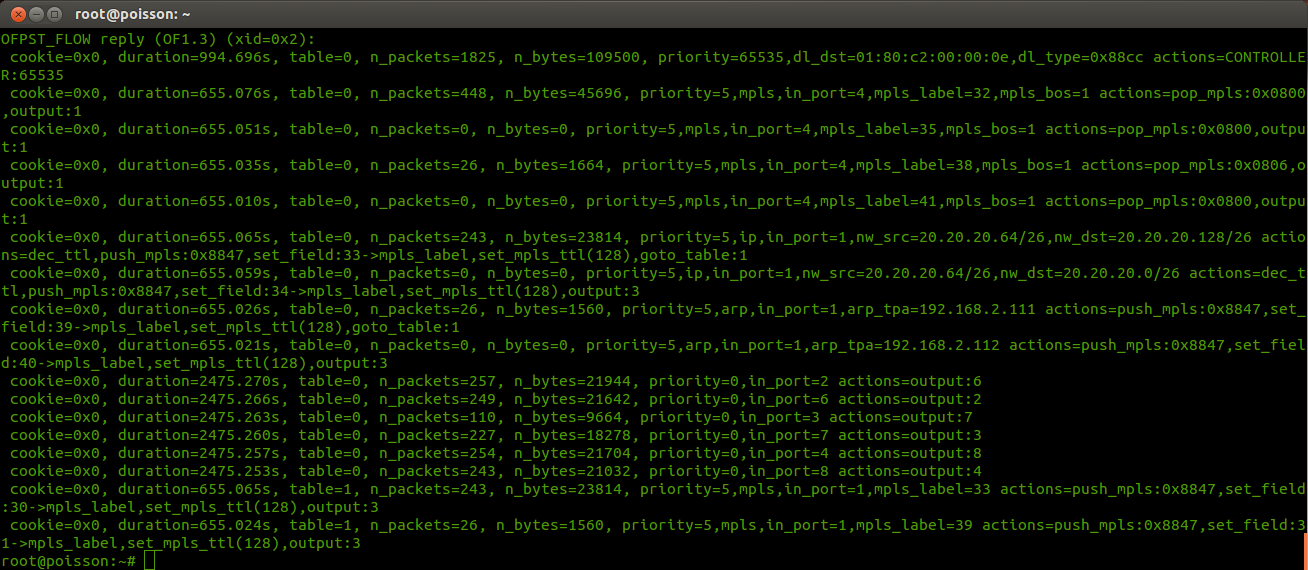
\includegraphics[width=1.0\textwidth]{LabE1P1Poi}
\caption[Tabla de flujos ovs - Poisson]{Tabla de flujos ovs - Poisson}
\label{fig:CU1P1DumpFlows3}
\end{figure}

\begin{figure}[ht!] 
\centering    
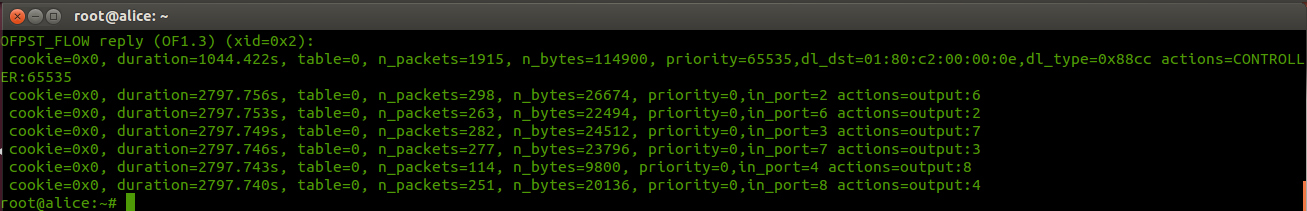
\includegraphics[width=1.0\textwidth]{LabE1P1Al}
\caption[Tabla de flujos ovs - Alice]{Tabla de flujos ovs - Alice}
\label{fig:CU1P1DumpFlows4}
\end{figure}


En otras palabras todo tr\'afico IP con origen en la subred A y destino a la subred B, es encaminado a través de la interfaz $nf_2$ en el nodo de ingreso \textit{Galois}. Luego en el nodo de egreso \textit{Poisson} es reenviado por la correspondiente interfaz del servicio.\\

Analizando las tablas de flujos de los nodos \textit{Galois} y \textit{Poisson}, puede comprobarse fácilmente la correspondencia entre el camino calculado y el camino te\'orico.

Por un lado en la tabla de flujos de \textit{Galois} se tiene el siguiente flujo:

%Por un lado, acorde a la definci\'on del servicio, Galois debería reenviar todo tr\'afico de tipo \textbf{ip} que ingresa por la interfaz eth1(la cual se corresponde con el n\'umero de puerto openflow 1), con origen en la subred 20.20.20.64/26 y destino 20.20.20.0/64 por la interfaz nf1(la cual se corresponde con el n\'umero de puerto openflow 3).

\begin{center}
\textit{cookie=0.0, duration=531.354s, table=0, n\_packets=0, n\_bytes=0, priority=5, \\
ip,in\_port=1, nw\_src=20.20.20.128/26,nw\_dst=20.20.20.0/26 \\
actions=dec\_ttl,push\_mpls:0x8847,set\_field:30->mpls\_label,set\_mpls\_ttl(128),output:4}
\label{lst:flows1}
\end{center}

En pocas palabras este flujo toma todo paquete recibido por el puerto openflow identificado con el n\'umero 1(interfaz eth1), numeración IP origen 20.20.20.128/26(subred A) y destino 20.20.20.64/26 (subred B), decrementa el ttl del paquete, coloca un cabezal mpls con la etiqueta 32 y lo reenvía por el puerto openflow identificado con el n\'umero 4(interfaz nf2). Observar el valor de la etiqueta mpls colocado en el mismo para identificar el servicio(etiqueta interna). 

%Notese adem\'as la acci\'on \textbf{dec\_ttl} en el flujo. Esta acci\'on es utilizada en cada nodo de borde en la definici\'on de un servicio para decrementar el ttl de un paquete ip cada vez que ingresa a la red del prototipo (en este caso a la red del laboratorio). Observese tambi\'en el valor de la etiqueta mpls(34) colocado en el paquete para identificar el servicio(etiqueta interna).

Por otro lado, una vez que los paquetes asociados al servicio S3 llegan a nodo \textit{Poisson} ingresando por la interfaz nf2(puerto openflow n\'umero 4), debe ser retirada la etiqueta mpls interna y reenviarse a través de la interfaz eth1(puerto openflow n\'umero 1).

Este comportamiento es implementado en la tabla de flujos de Poisson mediante el siguiente flujo:

\begin{center}
\textit{cookie=0.0, duration=655.076s, table=0, n\_packets=0, n\_bytes=0, priority=5, \\
mpls,in\_port=4,mpls\_label=32,mpls\_bos=1 \\
actions=pop\_mpls:0x0800,output:1 }
\end{center}

De esta forma todos los paquetes asociados al servicio S3 son reenviados desde el nodo de ingreso Galois al nodo de egreso Poisson mediante un solo enlace utilizando un solo nivel de etiquetas mpls.\\

Analizando el camino que deben seguir los paquetes que atraviesan la red del laboratorio en el sentido inverso; es decir, desde la subred B hacia la subred A, se analiza el camino calculado para el tr\'afico asociado al servicio S4. 

El camino te\'orico para el tr\'afico asociado a dicho servicio es:

$$<(Poisson, nf_1), (Oz, nf_0)>$$ 

Este camino es implementado mediante los siguientes flujos en la tabla del nodo \textit{Poisson} por un lado:

\begin{center}
\textit{cookie=0.0, duration=655.065s, table=0, n\_packets=0, n\_bytes=0, priority=5, \\
ip,in\_port=1, nw\_src=20.20.20.64/26,nw\_dst=20.20.20.128/26 \\
actions=dec\_ttl,push\_mpls:0x8847,set\_field:33->mpls\_label,set\_mpls\_ttl(128), goto\_table:1 \\
cookie=0.0, duration=655.065s, table=0, n\_packets=0, n\_bytes=0, priority=5, \\
mpls,in\_port=1,mpls\_label=33 actions=push\_mpls:0x8847,set\_fied:30->mpls\_label,set\_mpls\_ttl(128),output:3
}
\end{center}

Notar como primera diferencia en comparación con el camino anterior, que en este caso se tienen dos flujos: un primer flujo para colocar la etiqueta asociada al servicio (etiqueta interna) y un segundo flujo para colocar la etiqueta de reenvío (etiqueta externa). El camino anterior carece de etiqueta externa puesto que al ser un camino de un solo salto, el primer nodo coincide con el pen\'ultimo, y al implementar PHP no se coloca etiqueta externa. 

En pocas palabras se le colocan dos cabezales mpls al paquete y se reenvía a trav\'es del puerto n\'umero 3(interfaz nf1).\\

Al llegar al nodo \textit{Oz}, el siguiente salto en el camino es implementado por el siguiente flujo en la tabla de dicho nodo:

\begin{center}
\textit{cookie=0.0, duration=610.380s, table=0, n\_packets=243, n\_bytes=25748, priority=5, \\
mpls,in\_port=3,mpls\_label=30,mpls\_bos=0 actions=pop\_mpls:0x8847,output:2 }
\end{center}

Se le coloca una nueva etiqueta mpls externa con el valor 30, y se reenvia por el puerto n\'umero 4(interfaz nf2).\\

Finalmente en el nodo \textit{Galois} el tramo final del camino es implementado por el siguiente flujo en su tabla:

\begin{center}
\textit{cookie=0.0, duration=531.341s, table=0, n\_packets=234, n\_bytes=23868, priority=5, \\
mpls,in\_port=2,mpls\_label=33,mpls\_bos=1 actions=pop\_mpls:0x0800,output:1 }
\end{center}

Análogamente el lector puede completar el análisis de la correspondencia entre los caminos te\'oricos y los calculados por el algoritmo de ruteo. A continuaci\'on se analiza el algoritmo de distribucion de etiquetas.

\subsubsection{Verificaci\'on de Algoritmo de distribución de etiquetas}

[De repente comentar en funcion al escenario anterior porque anda bien]

En la siguiente secci\'on se analiza la clasificaci\'on de tr\'afico.

\subsubsection{Clasificaci\'on de tr\'afico}
Se implementa clasificaci\'on de tr\'afico en el nodo de borde identificado como ingreso para el tr\'afico de un servicio en particular. En particular, en el escenario definido se implementa clasificaci\'on de tr\'afico en basándose en la numeraci\'on IP origen y destino de un paquete. De esta forma por ejemplo el nodo Galois determina que camino debe tomar un paquete con origen en la Subred A y destino la Subred B. Luego en cada nodo intermedio los paquetes son procesados acorde a las reglas de reenvio en base a la conmutación de etiquetas mpls.

Para verificar el correcto funcionamiento de cada flujo OpenFlow involucrado en la clasificaci\'on de tr\'afico y en el posterior procesamiento del mismo para los paquetes de un servicio en particular, se elige un servicio y se observa el procesamiento de los paquetes asociados en cada nodo involucrado.\\

En la figura \ref{fig:LabE1P1CapsTraf} se muestra el procesamiento de los paquetes asociados al servicio S1 en cada uno de los nodos que atraviesa el camino construido, cuando se genera tr\'afico desde un host en la sub red A hacia otro host en la subred C.

Como puede observarse en el primer cuarto de la imagen (cuarto superior izquierdo), el cual se corresponde con una captura hecha con el comando \textbf{tcpdump} en la interfaz \textbf{eth1} del nodo \textit{Galois}, paquetes ICMP request con origen 20.20.20.131 y destino 20.20.20.05 son recibidos. Tambi\'en pueden observarse paquetes ICMP reply a los paquetes request.

Luego, como se muestra en el segundo cuarto de la imagen(cuarto superior derecho), el cual se corresponde con una captura del comando \textbf{tcpdump} en la interfaz nf0 del nodo \textit{Galois}, a cada paquete ICMP request se le coloca un cabezal mpls para luego ser reenviado por la interfaz \textbf{nf0}. Luego al arribar al nodo \textit{Oz} por la interfaz \textbf{nf0} de este nodo (cuarto inferior izquierdo de la imagen), el cabezal mpls es retirado de cada paquete para luego reenviarse por la interfaz \textbf{eth1} hacia la subred C (cuarto inferior derecho de la imagen).

\begin{figure}[ht!] 
\centering    
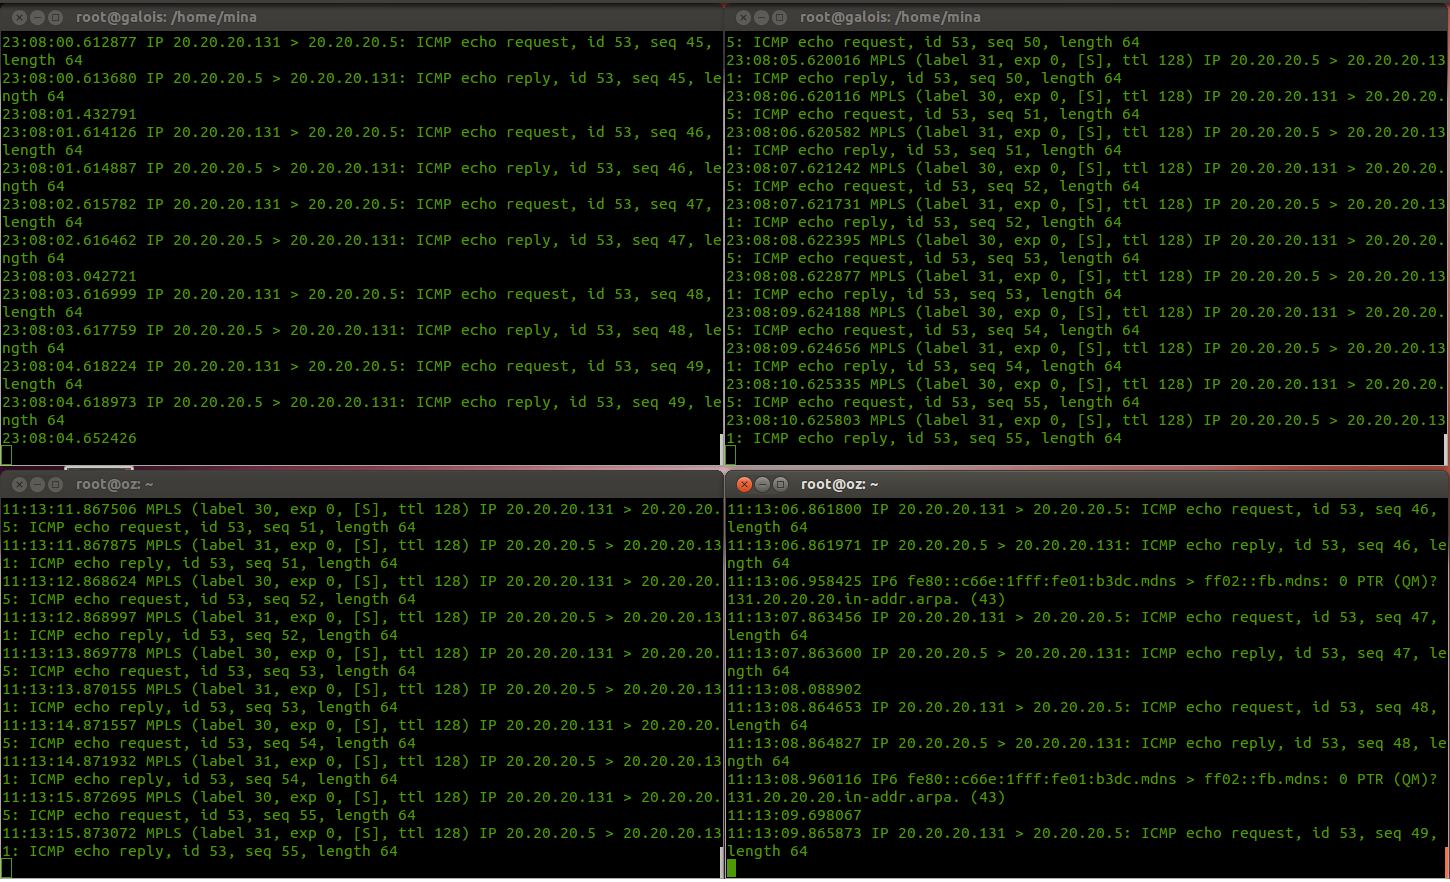
\includegraphics[width=1.0\textwidth]{LabE1P1CaputrasTrafico0}
\caption[Capturas de tr\'afico con tcpdump - servicio S1]{Capturas de tr\'afico con tcpdump - servicio S1}
\label{fig:LabE1P1CapsTraf}
\end{figure}

Finalmente en la figura \ref{fig:LabE1P1CapHost} puede verse una captura de pantalla del comando ping utilizado para generar tr\'afico ICMP desde el host 20.20.20.131 en la subred A, al host 20.20.20.05 en la subred C.

\begin{figure}[h!] 
\centering    
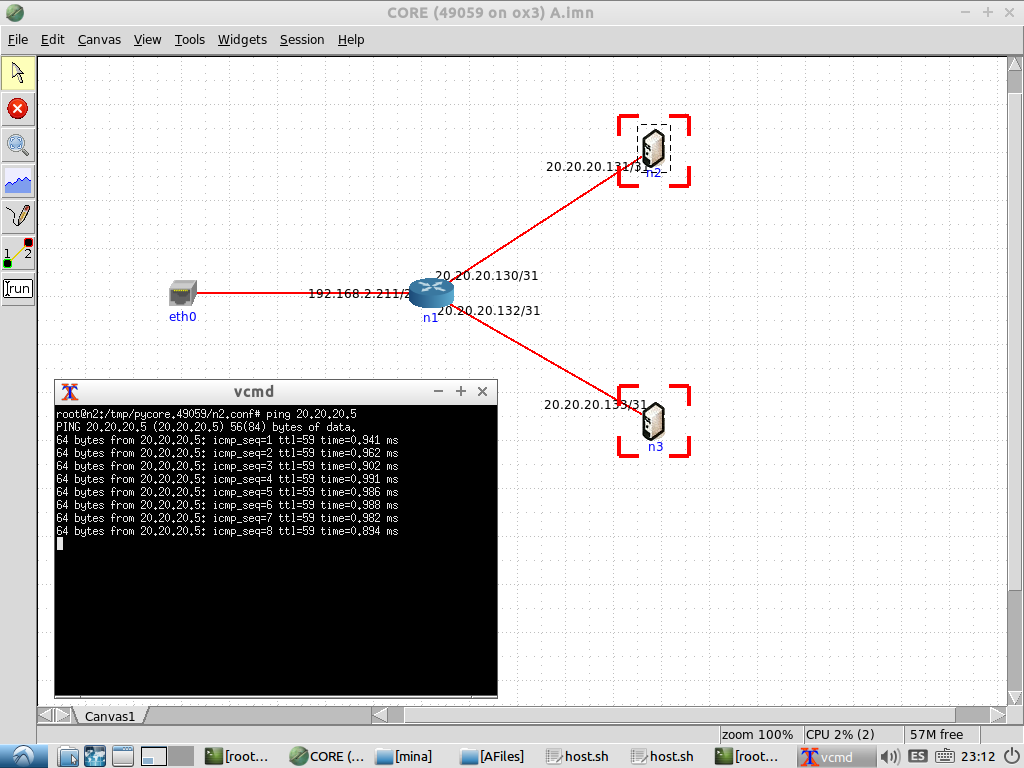
\includegraphics[width=0.6\textwidth]{E1P1202020131-2020205}
\caption[Capturas de comando ping H1-Subred A]{Capturas de comando ping H1-Subred A}
\label{fig:LabE1P1CapHost}
\end{figure}

Análogamente se procesan los paquetes asociados a los restantes servicios dados de alta en el sistema. En la figura \ref{fig:LabE1P1CapsTraf2} se muestra el procesamiento de paquetes asociados al servicio S3, cuando el host 20.20.20.131 en la sub red A envia paquetes ICMP al host 20.20.20.67 en la subred B, utilizando el comando tcpdump para realizar las capturas en la interfaz eth1(cuarto superior izquierdo de la imagen) y nf2(cuarto superior derecho de la imagen) del nodo Galois, y las interfaces nf2(cuarto inferior izquierdo) y eth1 (cuarto inferior derecho) del nodo Poisson.

\begin{figure}[ht!] 
\centering    
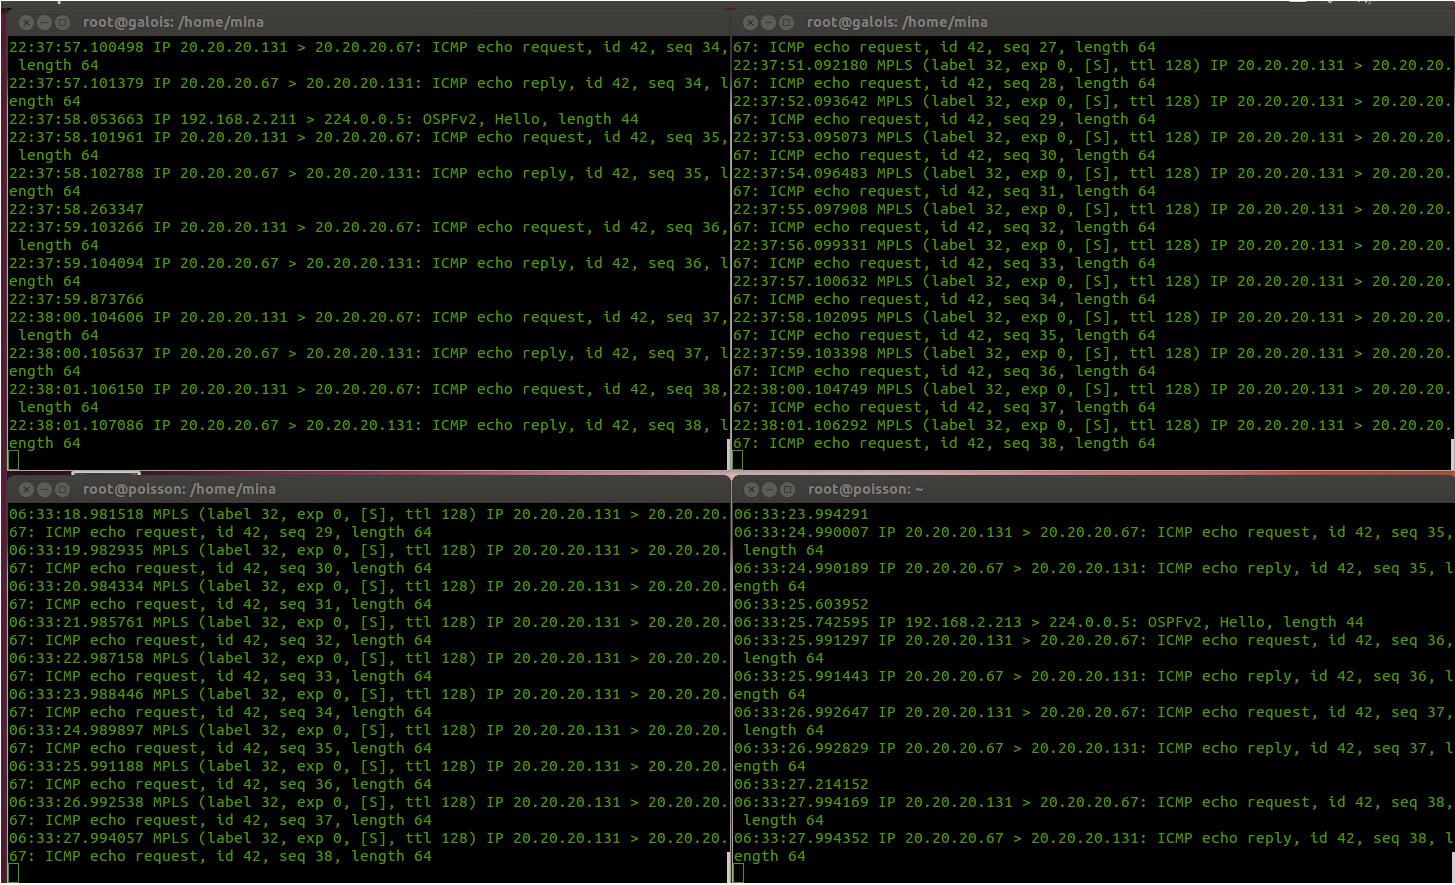
\includegraphics[width=1.0\textwidth]{LabE1P1CaputrasTrafico}
\caption[Capturas de tr\'afico con tcpdump - servicio S3]{Capturas de tr\'afico con tcpdump - servicio S3}
\label{fig:LabE1P1CapsTraf2}
\end{figure}

%Sin embargo RAUFlow admite realizar clasificaci\'on de tr\'afico por un conjunto bastante m\'as amplio de atributos. A continuaci\'on se definen una nueva lista de servicios orientados a demostrar la correcta implementaci\'on de esta funcionalidad.

%Cabe destacar que para esta prueba los servicios anteriormente creados son eliminados.

%\begin{table}[h]
%\begin{tabular}{| l | l | l | p{4cm} | p{4cm} |}
%\hline
%Nombre & Ingreso & Egreso & Clasificación & Descripción \\ \hline
%
%\crule[Aquamarine]{0.3cm}{0.3cm} S1 & Galois - eth1 & Oz - eth1 & ip\_src=20.20.20.128/26 ip\_dst=20.20.20.0/26 & Tr\'afico de Subred A a Subred C \\ \hline
%
%\crule[Red]{0.3cm}{0.3cm} S2 & Oz - eth1 & Galois - eth1 & ip\_src=20.20.20.0/26 ip\_dst=20.20.20.128/26 & Tr\'afico de Subred C a Subred A \\ \hline
%
%\crule[ForestGreen]{0.3cm}{0.3cm} S3 & Galois - eth1 & Poisson - eth1 & ip\_src=20.20.20.128/26 ip\_dst=20.20.20.64/26 & Tr\'afico de Subred A a Subred B \\ \hline
%
%\crule[LimeGreen]{0.3cm}{0.3cm} S4 & Poisson - eth1 & Galois - eth1 & ip\_src=20.20.20.64/26 ip\_dst=20.20.20.128/26 & Tr\'afico de Subred B a Subred A \\ \hline
%
%\crule[RoyalPurple]{0.3cm}{0.3cm} S5 & Poisson - eth1 & Oz - eth1 & ip\_src=20.20.20.64/26 ip\_dst=20.20.20.0/26 & Tr\'afico de Subred B a Subred C \\ \hline
%
%\crule[YellowOrange]{0.3cm}{0.3cm} S6 & Oz - eth1 & Poisson - eth1 & ip\_src=20.20.20.0/26 ip\_dst=20.20.20.64/26 & Tr\'afico de Subred C a Subred B \\ \hline
%\end{tabular}
%\vspace{0.3cm}

%\caption[CU1 - Escenario 1, servicios extra]{CU1 - Escenario 1, servicios extra}
%\label{table:TablaFlujos2}
%\end{table}

\newpage
\subsubsection{Actualizaci\'on de rutas}
Para probar la actualizaci\'on de rutas cuando cambia la topolog\'ia se trabaja nuevamente con los servicios definidos en \ref{table:TablaFlujos}. 

Una vez configurado el laboratorio de esta forma, se procede a derribar manualmente los enlaces $<(Galois, nf_2), (Poisson, nf_2)>$ y $<(Poisson, nf_2), (Poisson, nf_2)>$. De esta forma se produce una actualizaci\'on de la topolog\'ia tras la cual se ejecutan los algoritmos de ruteo y distribución de etiquetas para actualizar cada LSP.\\

Acorde a los costos de la topolog\'ia (ver figura \ref{fig:LaboratorioDePruebasCostos}), los nuevos caminos te\'oricos asociados a cada servicio, tras la actualziaci\'on son los siguientes:

\newpage
\begin{figure}[ht!] 
\centering    
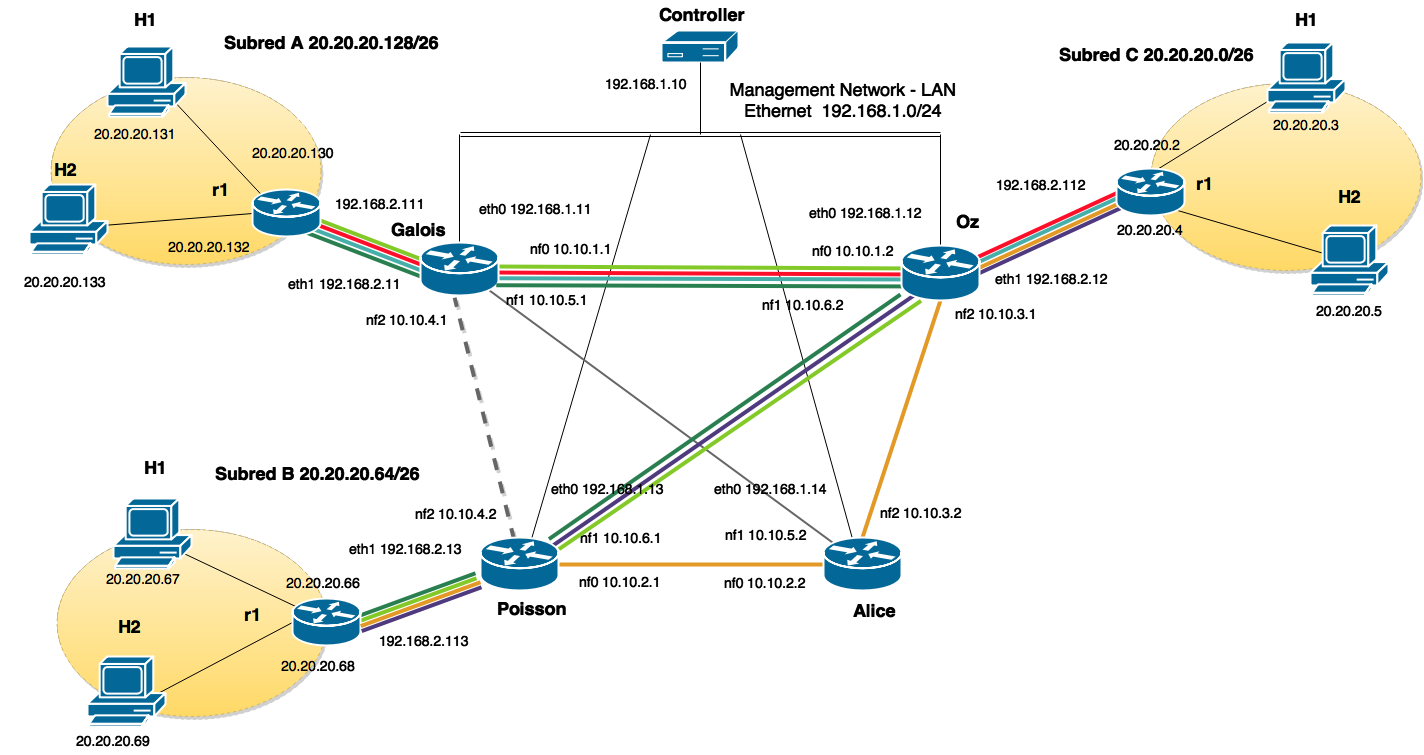
\includegraphics[width=1.0\textwidth]{CU1P1CaminosRecalculo}
\caption[Escenario 1 - Caminos para servicios recalculados]{Escenario 1 - Caminos para servicios recalculados}
\label{fig:CUP1Caminos2}
\end{figure}
 
Notese que los \'unicos caminos que cambian son los asociados a los servicios S3 y S6. Cabe destacar adem\'as que en la nueva topolog\'ia existe m\'as de un camino de m\'inimo costo para S3. Los caminos $<(Galois, nf0), (Oz, nf1)>$ y $<(Galois, nf0), (Oz, nf2), (Alice, nf0)>$ presentan ambos el costo 4.
Por tanto se tienen dos resultados v\'alidos posibles para la salida del algoritmo de ruteo para este servicio.\\

Para comprobar que el algoritmo de ruteo recaclula correctamente las rutas, se inspeccionan nuevamente las tablas de flujos de cada nodo en el laboratorio (ver figuras \ref{fig:CU1P2DumpFlows1}-\ref{fig:CU1P2DumpFlows4}), comparando los caminos calculados con los caminos te\'oricos.

\newpage
\begin{figure}[ht!] 
\centering    
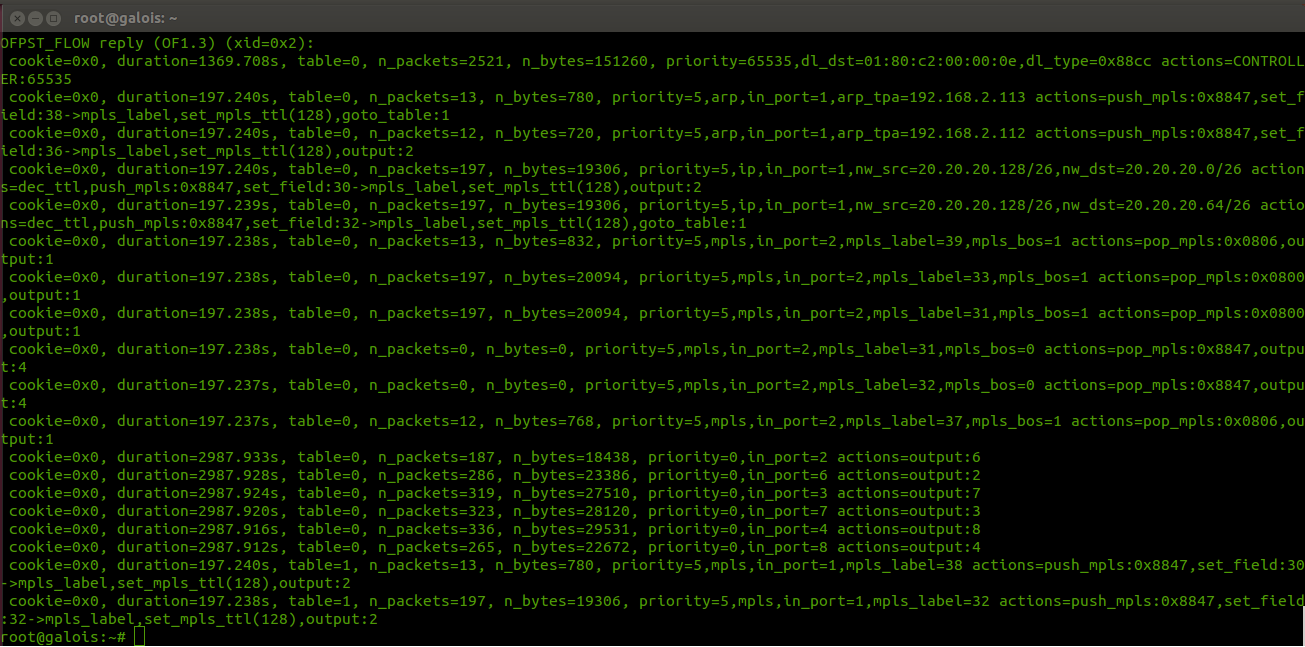
\includegraphics[width=1.0\textwidth]{LabE1P2Gal}
\caption[Tabla de flujos ovs - Galois]{Tabla de flujos ovs - Galois}
\label{fig:CU1P2DumpFlows1}
\end{figure}

\begin{figure}[h] 
\centering    
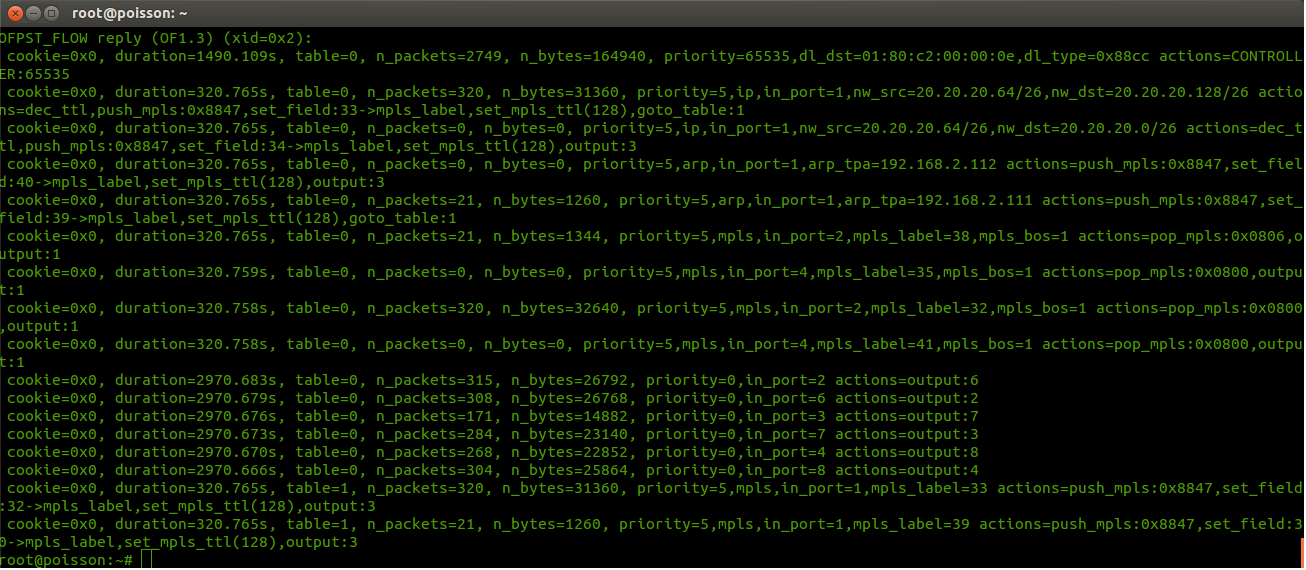
\includegraphics[width=1.0\textwidth]{LabE1P2Poi}
\caption[Tabla de flujos ovs - Poisson]{Tabla de flujos ovs - Poisson}
\label{fig:CU1P2DumpFlows3}
\end{figure}

\begin{figure}[h] 
\centering    
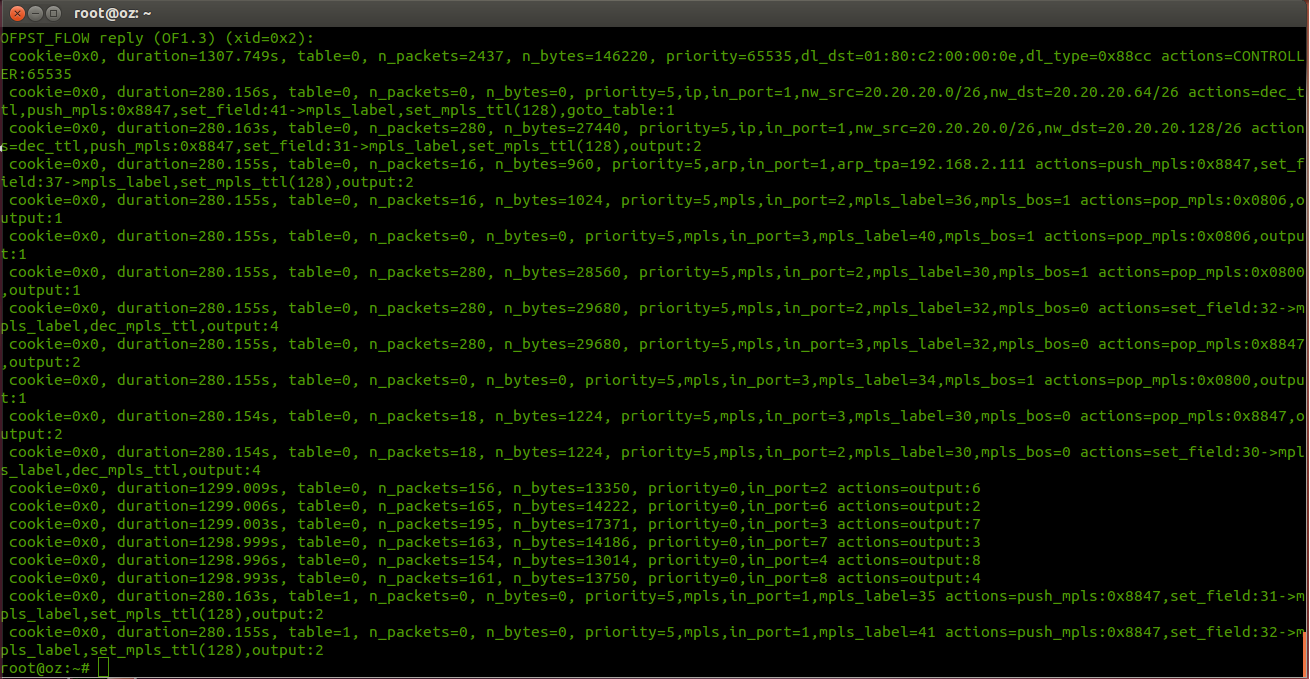
\includegraphics[width=1.0\textwidth]{LabE1P2Oz}
\caption[Tabla de flujos ovs - Oz]{Tabla de flujos ovs - Oz}
\label{fig:CU1P2DumpFlows2}
\end{figure}

\begin{figure}[h] 
\centering    
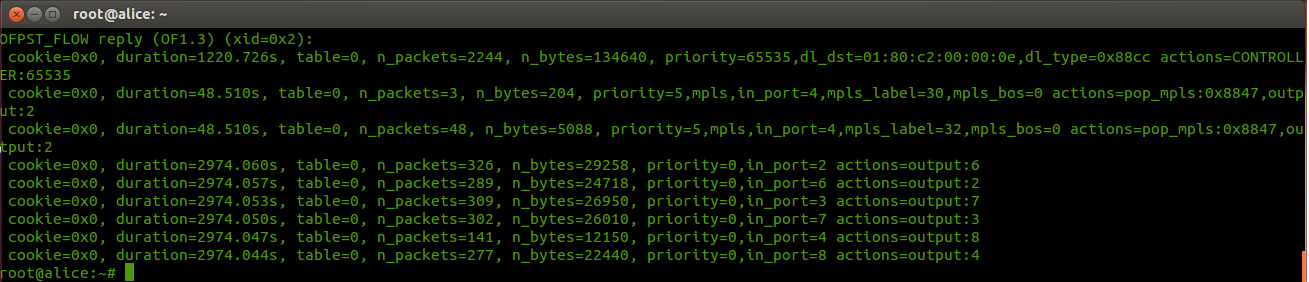
\includegraphics[width=1.0\textwidth]{LabE1P2Al}
\caption[Tabla de flujos ovs - Alice]{Tabla de flujos ovs - Alice}
\label{fig:CU1P2DumpFlows4}
\end{figure}

\newpage
Tomando como ejemplo la actualizaci\'on del LSP asociado al servicio S3, mientras que en la topolog\'ia original el camino asociado es $<(Galois, nf2)>$, tras la actualizaci\'on de la topolog\'ia el camino puede ser o bien $<(Galois, nf0),(Oz, nf1)>$ o bien \\ $<(Galois, nf0), (Oz, nf2), (Alice, nf0)>$.\\

Recordando la tabla de flujos original del nodo \textit{Galois}(ver imagen \ref{fig:CU1P1DumpFlows1}), el flujo \ref{lst:flows1} es el utilizado para procesar y reenviar paquetes al nodo Poisson. Al cambiar el camino asociado a S3, este flujo tambi\'en cambia. 

\newpage
\subsection{Escenario 2}

Este escenario representa una red privada punto a punto de capa 3. Esta compuesto por dos organizaciones diferentes, cada una de ellas con dos sucursales f\'isicamente separadas. Adicionalmente  ambas organizaciones utilizan la misma numeraci\'on IP en sus respectivas subredes.\\

\begin{figure}[ht!] 
\centering    
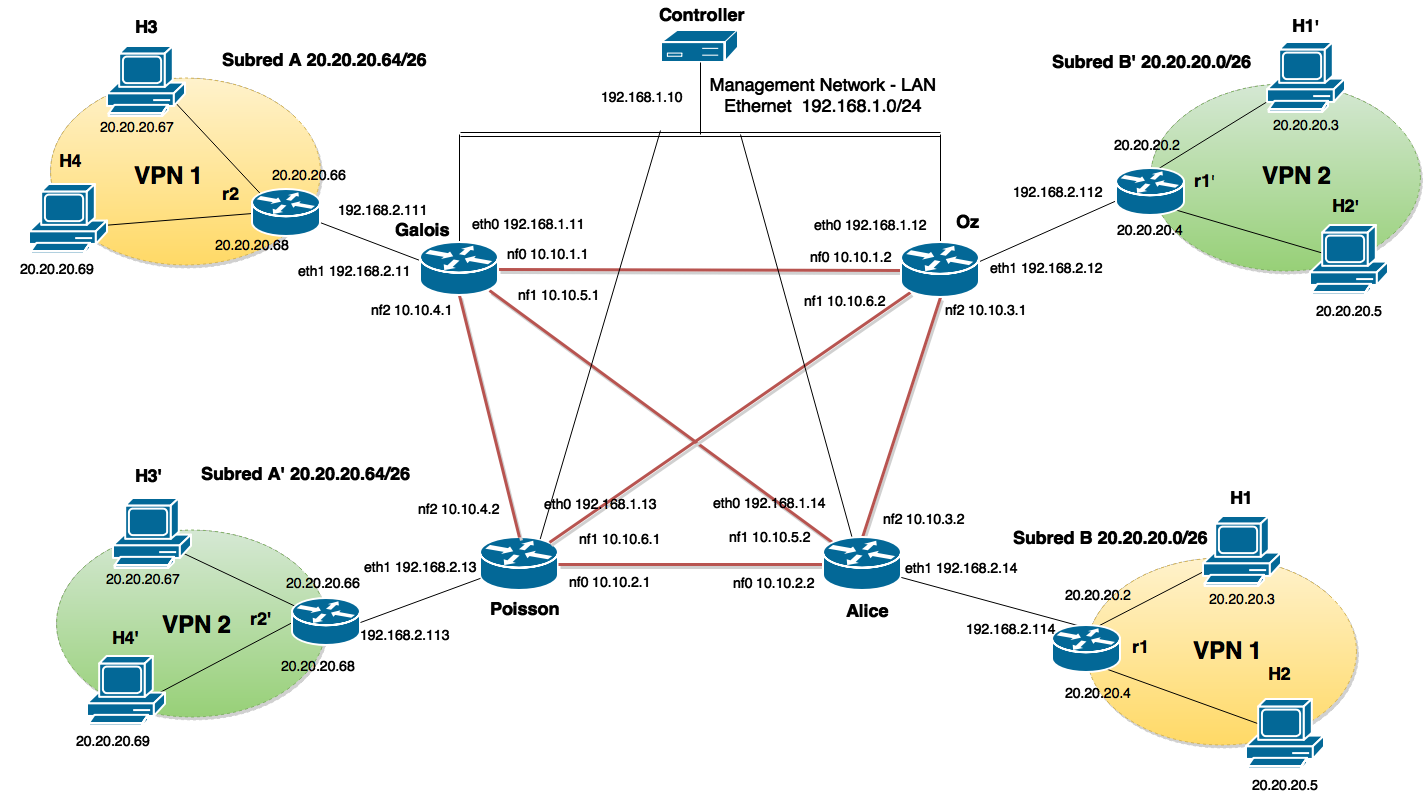
\includegraphics[width=1.0\textwidth]{CU1P2}
\caption[VPN de capa 3 - Escenario 2]{VPN de capa 3 - Escenario 2}
\label{fig:CUP2}
\end{figure}

Para la construcci\'on de este escenario se instancian los siguientes servicios en el sistema (ver tabla). Por cada red privada se instancian dos servicios (uno para cada sentido del tr\'afico).

\begin{table}[h]
\begin{tabular}{| l | l | l | p{4cm} | p{4cm} |}
\hline
Nombre & Ingreso & Egreso & Clasificación & Descripción \\ \hline

\crule[Aquamarine]{0.3cm}{0.3cm} S1 & Galois - eth1 & Alice - eth1 & ip\_src=20.20.20.64/26 ip\_dst=20.20.20.0/26 & Tr\'afico de Subred A a Subred B \\ \hline

\crule[Red]{0.3cm}{0.3cm} S2 & Alice - eth1 & Galois - eth1 & ip\_src=20.20.20.0/26 ip\_dst=20.20.20.64/26 & Tr\'afico de Subred B a Subred A \\ \hline

\crule[ForestGreen]{0.3cm}{0.3cm} S3 & Poisson - eth1 & Oz - eth1 & ip\_src=20.20.20.64/26 ip\_dst=20.20.20.0/26 & Tr\'afico de Subred A' a Subred B' \\ \hline

\crule[LimeGreen]{0.3cm}{0.3cm} S4 & Oz - eth1 & Poisson - eth1 & ip\_src=20.20.20.0/26 ip\_dst=20.20.20.64/26 & Tr\'afico de Subred B' a Subred A' \\ \hline

\end{tabular}
\vspace{0.3cm}
\caption[CU1 - Escenario 2]{CU1 - Escenario 2}
\label{table:TablaFlujos2}
\end{table}


\newpage
\begin{figure}[ht!] 
\centering    
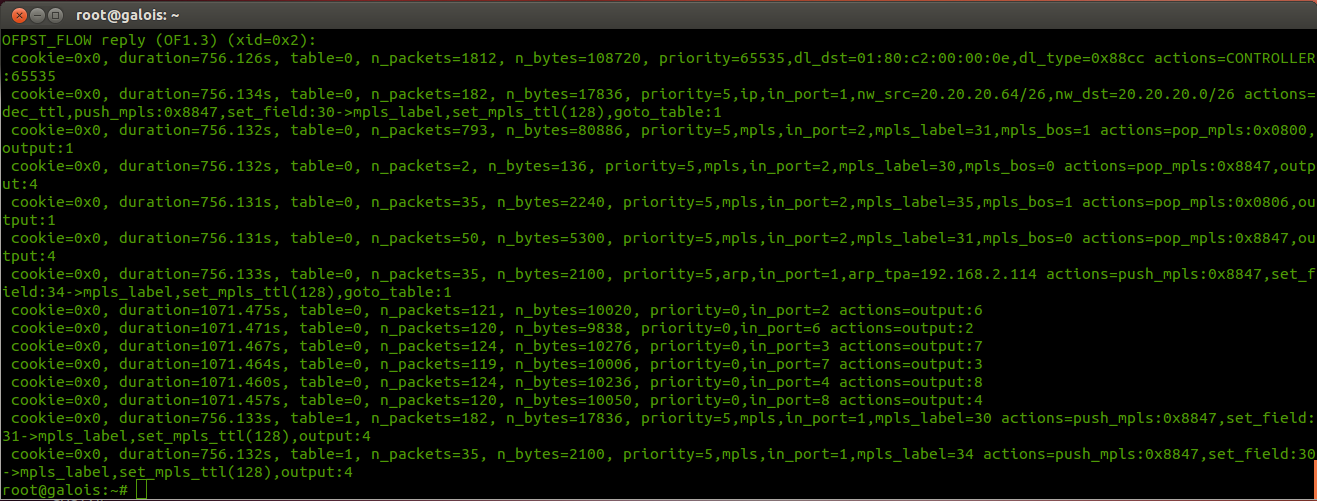
\includegraphics[width=1.0\textwidth]{E2P1Gal}
\caption[Tabla de flujos ovs - Galois]{Tabla de flujos ovs - Galois}
\label{fig:CU1P1DumpFlows1}
\end{figure}

\begin{figure}[h!] 
\centering    
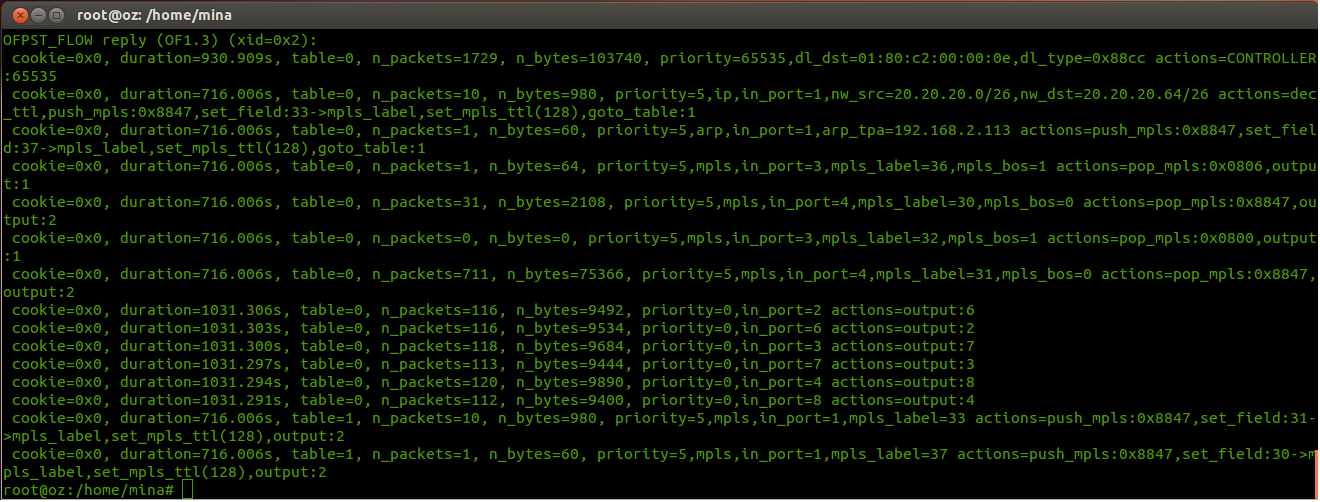
\includegraphics[width=1.0\textwidth]{E2P1Oz}
\caption[Tabla de flujos ovs - Oz]{Tabla de flujos ovs - Oz}
\label{fig:CU1P1DumpFlows2}
\end{figure}

\begin{figure}[h!] 
\centering    
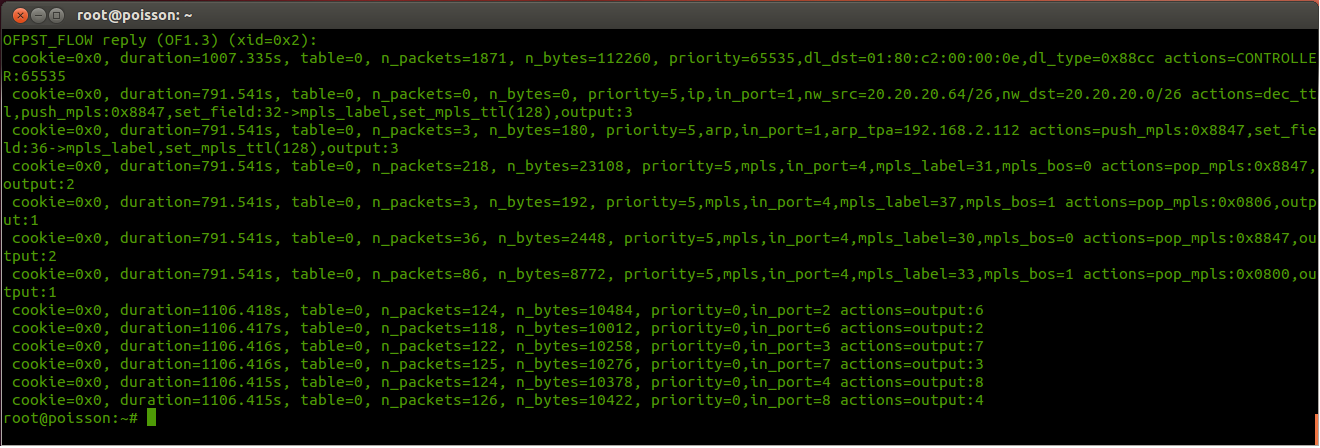
\includegraphics[width=1.0\textwidth]{E2P1Poi}
\caption[Tabla de flujos ovs - Poisson]{Tabla de flujos ovs - Poisson}
\label{fig:CU1P1DumpFlows3}
\end{figure}

\begin{figure}[h!] 
\centering    
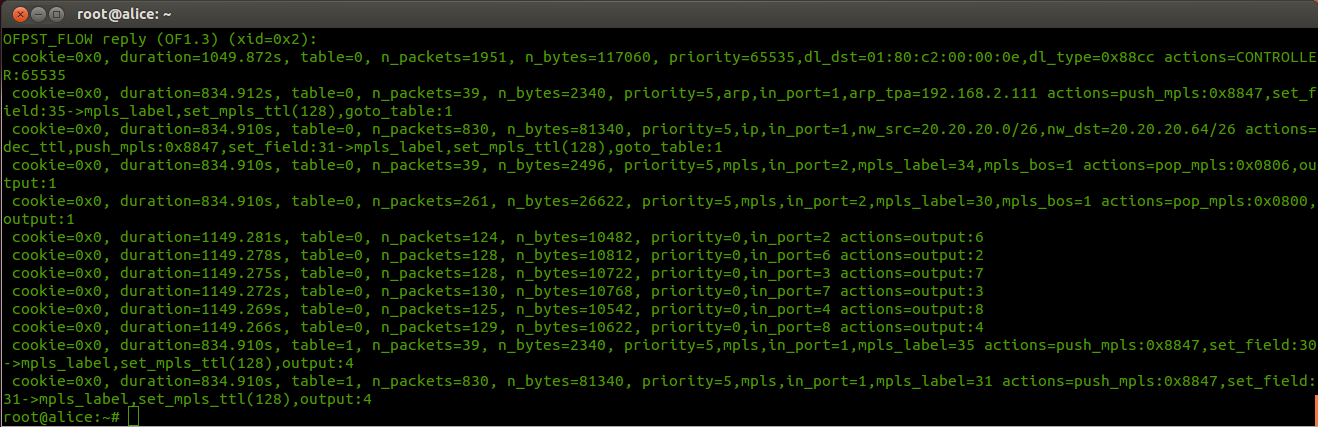
\includegraphics[width=1.0\textwidth]{E2P1Al}
\caption[Tabla de flujos ovs - Alice]{Tabla de flujos ovs - Alice}
\label{fig:CU1P1DumpFlows4}
\end{figure}

llalala

\newpage
\section{VPN de capa 2}
